\RequirePackage{fix-cm}
\documentclass[a4paper,ngerman]{scrartcl}

\usepackage[utf8]{inputenc}
\usepackage{cmbright}
\usepackage[T1]{fontenc}
\usepackage{babel}

\usepackage{paralist}	
\usepackage{geometry}	
\usepackage{tabularx}		
\usepackage{listings} 
\usepackage{datetime} 
\usepackage{graphicx}
\usepackage{enumitem}
\usepackage{booktabs}
\usepackage{multirow}
\usepackage{newunicodechar} 

\usepackage{color}
\usepackage{varioref} 
\usepackage[colorlinks=false, pdfborder={0 0 0}]{hyperref} 
\usepackage{cleveref} 

\setcounter{secnumdepth}{2} 
  
\definecolor{bluekeywords}{rgb}{0,0,1}
\definecolor{greencomments}{rgb}{0,0.5,0}
\definecolor{redstrings}{rgb}{0.64,0.08,0.08}
\definecolor{xmlcomments}{rgb}{0.5,0.5,0.5}
\definecolor{types}{rgb}{0.17,0.57,0.68}

\usepackage{listings}
\lstset{language=[Sharp]C,
	captionpos=b,
	showspaces=false,
	showtabs=false,
	breaklines=true,
	showstringspaces=false,
	breakatwhitespace=true,
	escapeinside={(*@}{@*)},
	commentstyle=\color{greencomments},
	morekeywords={partial, var, value, get, set, namespace},
	keywordstyle=\color{bluekeywords},
	stringstyle=\color{redstrings},
	basicstyle=\ttfamily\small,
	extendedchars=\true,
}

\begin{document}
\title{Amazing Race}
\subtitle{MOC5-Projekt}
\author{Stefan Kert}
\date{\today}
\maketitle

\section{Lösungsidee}
Als Plattform für die Projektarbeit wurde Windows Phone 8.1 gewählt, entwickelt wurde mit Visual Studio 2015 und dem dazugehörigen Emulator (WP8.1, 1GB RAM).
\subsection{Anwendungsstruktur}
\label{cha:Anwendungsstruktur}
Grundsätzlich besteht die \textit{AmazingRace}-App aus 3 Pages:
\begin{itemize}
	\item \textbf{LoginPage}: Hier erfolgt der Login. Falls die Zugangsdaten nicht erfolgreich sind, wird dem User eine entsprechende Fehlermeldung angezeigt.
	\item \textbf{RoutesPage}: Bietet eine Übersicht über alle verfügbaren Schnitzeljagd-Routen und die Möglichkeit, alle Routen zurückzusetzen. Diese Reset-Funktionalität wurde über einen AppBar-Button realisiert. Die verfügbaren Routen werden mit einem Icon in einer ListView angezeigt.
	\item \textbf{RouteDetailsPage}: Nachdem eine Route ausgewählt wurde, werden hier Details dazu angezeigt. Die Seite zeigt einerseits Titel und Hinweis des nächsten Checkpoints, und andererseits eine Karte, auf der dieser markiert ist. Außerdem wird die bereits zurückgelegte Route inkl. aller bisherigen Checkpoints auf der Karte eingezeichnet.
	
Außerdem kann der User über einen Button einen ContentDialog öffenen, indem die "`Secret"'-Passwortphrase für den nächsten Checkpoint eingetragen werden kann. Falls diese korrekt ist, werden sofort alle Details für den nächsten Checkpoint angezeigt.

Beim Abschluss einer Route (bzw. wenn der User zu einer Route navigiert, die bereits abgeschlossen ist) wird eine Erfolgsmeldung in Form eines MessageDialog eingeblendet und der User kann seinen zurückgelegten Weg nochmals auf der Karte betrachten.
\end{itemize}
\subsection{Implementierungsdetails}
\subsubsection{Architektur}
Die Anwendung setzt das für Windows-Anwendungen und -Apps typische MVVM-Muster um; das bedeutet, dass es zu jeder der drei in Abschnitt~\ref{cha:Anwendungsstruktur} beschriebenen Views ein entsprechendes ViewModel gibt. Dieses kennt die Views nicht, sondern bietet Datenkomponenten und Commands an, an die sich die View binden kann. Die Oberfläche bleibt dadurch austauschbar, ohne die Business Logic verändern zu müssen -- diese könnte ohne großen Aufwand z.B. auch für eine Windows-Desktopanwendung verwendet werden (Abb.~\ref{fig:arch}). 

\begin{figure}[h]
\centering
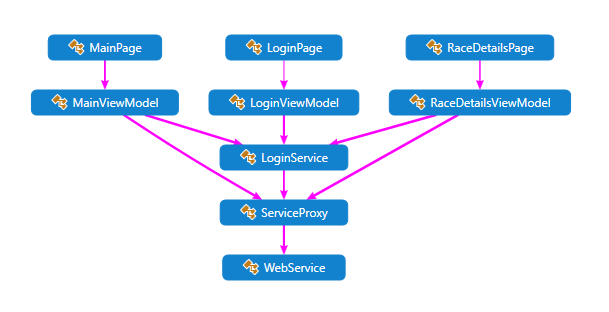
\includegraphics[width=.95\textwidth]{architecture}
\caption{Implementierung des MVVM-Patterns.}
\label{fig:arch}
\end{figure}

\subsubsection{Webservice-Anbindung}
Um die Applikation Daten mit dem Webservice austauschen zu lassen, wurde ein einfacher Service-Proxy entwickelt, der über einen \textit{HttpClient} GET- und POST-Requests ausführen und die Rückgabedaten direkt auf die entsprechenden Objekte mappen kann (für das Mapping wurde die von Microsoft empfohlene Bibliothek JSON.NET verwendet). Die Klasse \textit{ServiceProxy}, die das Interface \textit{IServiceProxy} implementiert, stellt dazu komfortable Methoden zur Verfügung. 

Die Login-Funktionalität wurde zudem noch in eine Klasse gekapselt, die das Singleton-Pattern implementiert (\textit{LoginService}). Dies stellt sicher, dass jede Page den Login-Status sowie die Benutzerdaten verwenden kann -- sollte eine Page aufgerufen werden, ohne dass ein User eingeloggt ist, wird der Benutzer auf die Login-Page weitergeleitet.

\subsubsection{Lifecycle-Management}
Der Lifecycle von Windows Phone 8.1-Apps ist prinzipiell dem von WP8 sehr ähnlich, allerdings gibt es kein \textit{Application-Deactivated}-Event mehr -- in WP8.1 werden Apps nicht mehr deaktiviert oder beim Verlassen beendet, sondern in den \textit{Suspended}-Status versetzt. Trotzdem kann die App bei Speicherknappheit beendet werden, dies geschieht ohne weitere Warnung.

Es muss also bei jedem Übergang in den \textit{Suspended}-Zustand angenommen werden, dass die App terminiert werden könnte. Um den Zustand der App zu persistieren, exisitert ein dem von WP8 bekannten State-Dictionary ähnliches Konstrukt: das \textit{SessionState}-Dictionary in der Klasse \textit{SuspensionManager}, die zudem noch die Möglichkeit, den Zustand eines Frames zu persistieren, enthält. Diese Funktionalität wird benutzt, um den Login-Status der App beizubehalten und die Login-Seite falls nötig zu überspringen.


\newpage
\section{Use Cases}
\subsection{Login mit falschem Benutzernamen/Kennwort}
Bei Eingabe eines falschen Benutzernamens oder Kennworts erfolgt kein Login und der Benutzer wird benachrichtigt.

\begin{figure}[h]
\centering
\includegraphics[width=.95\textwidth]{screenshots/login-error}
\caption{Login-Bildschirm vor und nach fehlgeschlagenem Login.}
\label{fig:GraphDb}
\end{figure}

\newpage
\subsection{Login mit richtigem Benutzernamen und Kennwort}
Bei Eingabe eines korrekten Benutzernamens und dazu passenden Kennworts erfolgt der Login und der Benutzer wird auf die Routenübersicht weitergeleitet.


\begin{figure}[h]
\centering
\includegraphics[width=.95\textwidth]{screenshots/login-success}
\caption{Erfolgreicher Login-Ablauf.}
\label{fig:GraphDb}
\end{figure}

\newpage
\subsection{Auswahl einer Route und erfolgreiches Freischalten eines Checkpoints}
Der Benutzer kann auf der Routen-Übersichts-Seite eine Route auswählen und wird dann auf die Detail-Seite weitergeleitet. Auf dieser kann er über den entsprechenden Button den nächsten Checkpoint freischalten -- nach einem Klick auf diesen wird dazu ein Dialog gezeigt. Bei richtiger Eingabe wird die Detail-Seite aktualisiert.


\begin{figure}[h]
\centering
\includegraphics[width=.95\textwidth]{screenshots/route-successfull}
\caption{Erfolgreicher Login-Ablauf.}
\label{fig:GraphDb}
\end{figure}

\subsection{Auswahl einer Route und nicht erfolgreiches Freischalten eines Checkpoints}
Der Benutzer kann auf der Routen-Übersichts-Seite eine Route auswählen und wird dann auf die Detail-Seite weitergeleitet. Auf dieser kann er über den entsprechenden Button den nächsten Checkpoint freischalten -- nach einem Klick auf diesen wird dazu ein Dialog gezeigt. Bei falscher Eingabe wird die Detail-Seite nicht aktualisiert.


\begin{figure}[h]
\centering
\includegraphics[width=.95\textwidth]{screenshots/route-failure}
\caption{Erfolgreicher Login-Ablauf.}
\label{fig:GraphDb}
\end{figure}


\newpage
\section{Quellcode}

\subsection{Views}
\lstinputlisting
[caption=LoginPage.xaml]
{../AmazingRace/AmazingRace/Views/LoginPage.xaml}

\lstinputlisting
[caption=LoginPage.xaml.cs]
{../AmazingRace/AmazingRace/Views/LoginPage.xaml.cs}

\lstinputlisting
[caption=RouteDetailsPage.xaml]
{../AmazingRace/AmazingRace/Views/RouteDetailsPage.xaml}

\lstinputlisting
[caption=RouteDetailsPage.xaml.cs]
{../AmazingRace/AmazingRace/Views/RouteDetailsPage.xaml.cs}

\lstinputlisting
[caption=RoutesPage.xaml]
{../AmazingRace/AmazingRace/Views/RoutesPage.xaml}

\lstinputlisting
[caption=RoutesPage.xaml.cs]
{../AmazingRace/AmazingRace/Views/RoutesPage.xaml.cs}

\lstinputlisting
[caption=UnlockCheckpointDialog.xaml]
{../AmazingRace/AmazingRace/Views/UnlockCheckpointDialog.xaml}

\lstinputlisting
[caption=UnlockCheckpointDialog.xaml.cs]
{../AmazingRace/AmazingRace/Views/UnlockCheckpointDialog.xaml.cs}


\subsection{ViewModels}
\lstinputlisting
[caption=ViewModelBase.cs]
{../AmazingRace/AmazingRace/ViewModels/ViewModelBase.cs}

\lstinputlisting
[caption=LoginViewModel.cs]
{../AmazingRace/AmazingRace/ViewModels/LoginViewModel.cs}

\lstinputlisting
[caption=RouteDetailsViewModel.cs]
{../AmazingRace/AmazingRace/ViewModels/RouteDetailsViewModel.cs}

\lstinputlisting
[caption=RoutesViewModel.cs]
{../AmazingRace/AmazingRace/ViewModels/RoutesViewModel.cs}


\subsection{Services}
\lstinputlisting
[caption=IServiceProxy.cs]
{../AmazingRace/AmazingRace/Services/IServiceProxy.cs}

\lstinputlisting
[caption=ServiceProxy.cs]
{../AmazingRace/AmazingRace/Services/ServiceProxy.cs}

\lstinputlisting
[caption=LoginService.cs]
{../AmazingRace/AmazingRace/Services/LoginService.cs}

\lstinputlisting
[caption=ServiceProxyFactory.cs]
{../AmazingRace/AmazingRace/Services/ServiceProxyFactory.cs}


\subsection{Converters}
\lstinputlisting
[caption=BooleanToVisiblityConverter.cs]
{../AmazingRace/AmazingRace/Converters/BooleanToVisiblityConverter.cs}
\end{document}
